% !TEX TS-program = xelatex
% !TEX encoding = UTF-8 Unicode
% !Mode:: "TeX:UTF-8"

\documentclass{resume}
\usepackage{zh_CN-Adobefonts_external} % Simplified Chinese Support using external fonts (./fonts/zh_CN-Adobe/)
%\usepackage{zh_CN-Adobefonts_internal} % Simplified Chinese Support using system fonts
\usepackage{linespacing_fix} % disable extra space before next section
\usepackage{cite}
\usepackage{tabu}
\usepackage{multirow}
\begin{document}
\pagenumbering{gobble} % suppress displaying page number

\Large{
  \begin{tabu}{ c l r }
   \multirow{4}{2in}{\hspace{1cm}\vspace{5mm}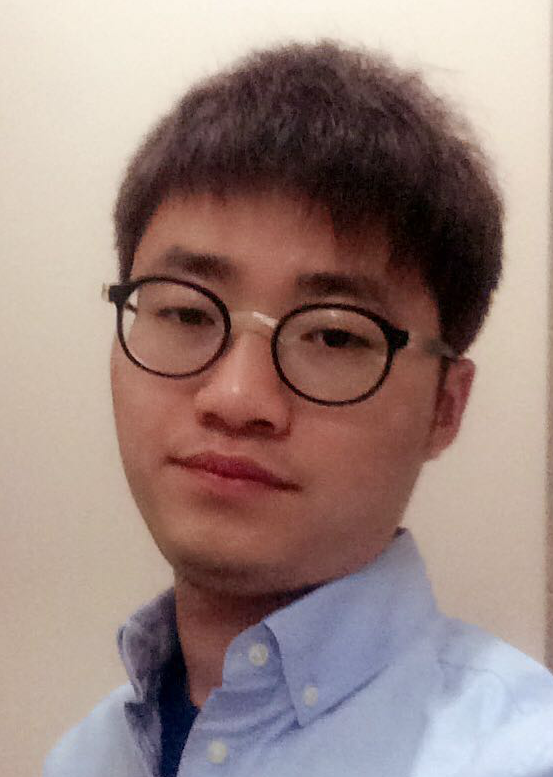
\includegraphics[width=1.1in, height =1.2in]{photo.png}} &\hspace{1cm}\Huge{\textbf{陈祺}}\\
    & \hspace{1cm}\email{chen147@usc.edu}  \\
    & \hspace{1cm}\phone{(+1) 213-479-3339}  \\
    & \hspace{1cm}\linkedin[Qi Chen]{https://www.linkedin.com/in/qi-chen-9a263a12a/}  \\
    
  \end{tabu}
}\\



%\name{陈祺}
%
%\basicInfo{
%  \email{chen147@usc.edu} \textperiodcentered\ 
%  \phone{(+1) 213-479-3339(美国号码)} \textperiodcentered\ 
%  \linkedin[LinkedIn]{https://www.linkedin.com/in/qi-chen-9a263a12a/}}
 
\section{\faGraduationCap\  教育背景}
\datedsubsection{\textbf{南加利福尼亚大学}, 洛杉矶}{08/2016 -- 05/2018}
\normalsize{\textit{在读硕士研究生}\ 计算机科学 -绩点: 4.0/4.0 (前 10\%)}
\datedsubsection{\textbf{南京邮电大学}, 南京}{09/2012 -- 06/2016}
\large{\textit{学士}}\ \normalsize{通信工程 -绩点: 3.71/4.0 (前 10\%)}

\vspace{-2mm}
\section{\faCogs\ IT 技能}
% increase linespacing [parsep=0.5ex]

\begin{itemize}[parsep=0.5ex]
  \item 编程语言: \hspace{2cm}JAVA, Python, Matlab, \LaTeX
  \item 其他技术: \hspace{2cm}SQL, HTML/CSS, Javascript, PHP, JSON, Linux
\end{itemize}

\vspace{-3mm}
\section{\faUsers\ 学术项目}
\datedsubsection{\textbf{多维能效云资源调度策略},南京}{09/2014 -- 05/2015}
\role{\hspace{6mm}导师: 陈建新副教授}{}
\vspace{-3mm}
\normalsize{
\begin{itemize}
  \item 提出了一个基于CPU利用率的虚拟机迁移算法,该算法平衡了数据中心物理机能耗和用户体 验QoS,将该问题转化为最优化问题,并使用禁忌算法得到全局优解
  \item 用java语言扩展了开源CloudSim云调度仿真平台,实验结果显示我们提出的算法比贪心算法 减少了75\%的虚拟机迁移和40\%的能耗
  \item 发表文章: \href{http://www-scf.usc.edu/~chen147/ICC\%20paper.pdf}{Qi Chen, et al. “Utilization-based VM consolidation scheme for power efficiency in cloud data centers” in Communication Workshop (ICC), 2015 IEEE International Conference on }
\end{itemize}
}

\vspace{-3mm}
\section{\faUsers\ 项目经历}
\datedsubsection{\textbf{国会议员搜索系统}, 洛杉矶}{01/2017 -- 05/2017}
%\begin{onehalfspacing}
\begin{itemize}
  \item 基于HMT/CSS, JS设计了一个用于搜索美国国会议员信息的网站
  \item 基于PHP开发了后端服务器脚本用于获取和处理从开源Sunlight API得到的JSON数据
  \item 部署该网页在Amazon Web Service(AWS)
\end{itemize}
%\end{onehalfspacing}

\datedsubsection{\textbf{人工智能课程项目},洛杉矶}{09/2016 -- 12/2016}
%\role{Golang, Linux}{个人项目,和富帅糕合作开发}
%\begin{onehalfspacing}
%分布式负载均衡科学上网姿势, https://github.com/cyfdecyf/cow
\begin{itemize}
  \item 基于DFS, BFS, Dijkstra和A*算法,实现了最短路径搜索策略
   \item 基于 Minmax和Alpha-Beta pruning算法,实现了人工智能棋盘游戏
\end{itemize}
%\end{onehalfspacing}

\datedsubsection{\textbf{智能防碰撞小车},南京}{09/2015 -- 12/2015}
%\role{\LaTeX, Python}{个人项目}
%\begin{onehalfspacing}
%优雅的 \LaTeX\ 简历模板, https://github.com/billryan/resume
\begin{itemize}
  \item 开发了一款防碰撞小车系统,小车根据周围动态环境来调整车速,并与前车保持一定距离
  \item 使用超声波和红外线传感器来为小车实现测距模块,并使用3D-Printing制造小车零部件
\end{itemize}
%\end{onehalfspacing}

\datedsubsection{\textbf{在线网络社交 Android APP},南京}{03/2013 -- 07/2013}
%\role{\LaTeX, Python}{个人项目}
%\begin{onehalfspacing}
%优雅的 \LaTeX\ 简历模板, https://github.com/billryan/resume
\begin{itemize}
  \item 开发了一款基于安卓平台的社交网络应用,实现了添加好友,聊天,发状态和评论等功能,
有两人一起开发这个APP,其中一人负责Android SDK界面部分开发,我负责后台服务器处理
  \item 设计了MySQL数据库表,使用Hibernate连接数据库,并运用Hibernate Query Language (HQL)
进行数据库搜索
  \item 基于Servlet, 获取用户请求并在后台进行处理请求,并运用百度云推送实现了信息推送功能
\end{itemize}
%\end{onehalfspacing}


% Reference Test
%\datedsubsection{\textbf{Paper Title\cite{zaharia2012resilient}}}{May. 2015}
%An xxx optimized for xxx\cite{verma2015large}
%\begin{itemize}
%  \item main contribution
%\end{itemize}


\section{\faHeartO\ 获奖情况}
\datedline{\textit{校一等奖学金} }{06/2015}
\datedline{\textit{三等奖}, 全国大学生挑战杯}{10/2015}


%% Reference
%\newpage
%\bibliographystyle{IEEETran}
%\bibliography{mycite}
\end{document}
